% !TeX root = muray.tex
% !TEX program = lualatex

\documentclass[14pt,oneside,american,a4paper]{memoir}
\usepackage[pdftitle=The Empire of the Good,pdflang=en-US,colorlinks=false,bookmarksopen=true,hidelinks]{hyperref}
\usepackage[T1]{fontenc}
\usepackage[utf8]{inputenc}
\usepackage{graphicx}
\usepackage{
	hyperxmp,bookmark,nameref,url,
	color,xcolor,microtype,keystroke,
	enumitem,fontspec,fancyhdr,titlesec,lipsum
}
\usepackage[english]{babel}
\newcommand\nbvspace[1][3]{\vspace*{\stretch{#1}}}
\newcommand\nbstretchyspace{\spaceskip0.5em plus 0.25em minus 0.25em}
\newcommand{\nbtitlestretch}{\spaceskip0.6em}
\definecolor{gray75}{gray}{0.75}
\newcommand{\hsp}{\hspace{20pt}}
\titleformat{\chapter}[hang]{\Huge\bfseries}{\thechapter\hsp\textcolor{gray75}{|}\hsp}{0pt}{\Huge\bfseries}


\title{The Empire of the Good}
\author{Philippe Muray}
\date{}
\begin{document}

\frontmatter
\pagestyle{empty}
\begin{center}
\bfseries
\nbvspace[1]
\Huge
{\nbtitlestretch\huge
The Empire of the Good}

\nbvspace[3]
\Large{Philippe Muray}

\nbvspace[3]
\includegraphics[width=11cm]{res/cover.jpg}

\nbvspace[3]
\footnotesize{Translated to English from the Original French by\\
Nadim Kobeissi}

\normalsize
%DOHA\\
%\large
%PUBLISHED IN THE WILD
\nbvspace[1]
\end{center}
\clearpage

\chapter*{Translator's Note}
\label{ch:notes}

Muray's \textit{L'Empire du Bien} was first published in October 1998, but like the rest of Muray's works, was never before translated into English.

The ISBN for the original French language edition of this work is 978-2-251-44393-5.

\begin{flushright}
	\textit{Nadim Kobeissi\\April 2020\\Paris, France.}
\end{flushright}
\clearpage

\pagestyle{fancy}
\fancyhf{}
\fancyhead[LE,RO]{The Empire of the Good}
\fancyfoot[LE,RO]{\thepage}
\chapter*{Preface: The Childhood of the Good}
\fancyhead[RE,LO]{Preface}
\label{ch:preface}
% 8 pages

The Good moves swiftly. It gallops forward. It climbs from all sides. It festers, grows, conquers terrain, recruits new missionaries at every opportunity. The Good grows rapidly -- little by little, permeating all exits and forbidding all escape routes. It is the Good that remakes the day and the night, the sun and the stars, space and time. Since the dawn of \textit{The Empire of the Good}, the Good has spiraled downwards. Seven little years were enough for the Good to sink, to stampede, to unfurl itself, carrying and dragging along with it all that it could find in its path, overturning any resistance that remained, overflowing from its bed, grazing its banks, hurtling on a train from hell -- or rather, from paradise -- spreading everywhere, blossoming, circulating, conquering and subjugating all that could still be tempted to oppose it.

Now, the Good has reached its objective, or almost -- and it loses itself deliciously in the immensity of its Festival, like a river into the sea that was long promised to it. And all that it has uprooted in its mad race, it now offers to the endless backwash in which it itself falls into ruin, like so many witnesses of their own common victory.

Together, now, the Good and the Festival, their powers combined, know no limit; and they melt into each other, to start, based on the invented power of their pretended enemies, the virulent dishonesty and archaic malfeasance of which these good apostles never cease to denounce. The Good, like the Festival, are ticklish, susceptible, irritable. They feed themselves on the sentiment of persecution. Having reduced all opposition to mutism does not suffice; they must still ceaselessly shake the scarecrow. And in the widespread silence of cowardice, of stupefaction and acquiescence, they must always fortify themselves against phantom attacks, puppet perils and adversarial simulacra.

In 1991, the Good was, for all intents and purposes, still in its childhood. It was still far from knowing the full extent of its powers. Nevertheless, it tried out its strengths, with the air of a hestitating infant; stammering, like a toddler that, certainly, was already monstrous and that benefitted from a concerningly strong bill of health, but with whom we could still envision a quelling through an accident, an illness, a cot death, something or another that could save humanity from the fatal peril of its rapid growth, from the weight of its irresistible extension.

In 1991, the Good seemed fragile, like a simple hypothesis, akin a supposition to which it was sufficient to cast a puzzled look at the right moment to discourage the worst of our kind from pursuing. The Good seemed timid, emotive, anxious vis-\'a-vis the sniggers that its initial philantrophic abuses could set off within a few free spirits, which indeed roamed free but were already under a state of precarious survival. And Cordicopolis, the city of rose-tinted nightmares which the Good was, to the applause of almost all, laying the foundations, still had only the allure of a half-baked utopia.

The Good, in 1991, was still in swaddling clothes, but this little Nero, this dictator of Altruism, already had serious assets on its side. It had already begun to expand its radiant prison around humanity and with humanity's consent. All of its predecessors, under the name of, for example, \textit{public welfare} -- with whatever this notion impliles in terms of an undifferentiated whole whose growth should be encouraged through the police, the justice system, and of course the prattle of the media, all only waiting to flourish thanks to it and to impose themselves in all areas of everyday existence. All that was left for the Good was for it to stream into the grand river of \textit{Amour-en-liesse}; and to admit into it the idea that the virtuous life is the festive life. The Good had flown straight in that direction. It had quickened itself, hasty, precipitously. It had only one goal, and it was clearly in approach.

In a general sense, most of the themes that I discussed in 1991 have not ceased to worsen, to darken still, even as they appear in colors that are more and more desirable to populations at large. The cordicoles\footnote{\textbf{Translator's note:} from the latin \textit{cor}, \textit{cordis} (``heart'') and \textit{-cole} (``he who veneres''), meant in a lightly deprecating tone.}, cordicolicians and cordophiles multipiled. Cordicologists, on the other hand, were not legion. And cordicoclasts (by which I mean the eventual demystifiers of cordicole norms) observed in silence. They observe in silence still. Since 1991, the actors of Transparency, those possessed by Homogeinity, the cursaders for the abolition of all differences and the raging bulls of retroactive trials launched themselves with a frenzy the good merits of which no one still dares to doubt. Operation ``Clean Record'' is almost accomplished. The demand for laws, which I at the time was still only sketching the pathology, and that I was then brought to define as a sort of \textit{penal envy}, had still not found its good rhythm, its groove, it still hadn't become the cry of extasy and resentment of millions of human ants to which judges, galvanized by the encouragement of the media herd offering the spectacle of the daily grind of their politicians. The demand for laws was also still not precisely the powerful accelerator of the \textit{change of attitude}\footnote{\textbf{Translator's note:} \textit{changement des mœurs}, which can also be translated as ``change of lifestyle'', ``change of behavior'', or ``change of habit'', especially moral habit.} that it was henceforth destined to be; neither was it still the ideal machine for criminalizing, with all its strength, all which did not have the ability or possibility to present itself \textit{on time} as a \textit{long-standing victim}. We had not yet, in 1991, opened the floodgates to the radiant wrongdoers of the penal code, nor to the squared knives of judiciary power. We had not quite yet, in 1991, changed the meaning of words to the point of seeing, without blinking, the worst consensual scoundrels fighting consensus, and the strongmen of neo-conformism rise with indignation against conformism. In 1991, it was still possible to be astonished at the spectacle rendered by so many beautiful souls going to battle (for the good causes), with an ardour that one could have seen, in other times, employed within more paradoxical, more perilous, more equivocal, and therefore more interesting theatres.

In 1991, those that I would call, a few years later, the \textit{truismocrats} (those men and women that fill with all the pathos in the world their fight against asbestos, p{\ae}dophilia, smoking, homophobia, xenophobia, having replaced the great fights-to-the-death of yesteryear with a dutiful humanitarian imposition to which they give the appearance of a perpetual crusade) had not yet set up their regular patrols, watching so that none remains estranged from their indefatigable exploits. In 1991, all of the \textit{bondieuseries}\footnote{\textbf{Translator's note:} a church ornament or devotional object, especially one of little artistic merit (i.e. a ``religious knick-knack''). Commonly found at gift shops inside large and well-known churches in Europe.} of generalized ``creolization'', that shepherd's idyll in the form of a new age archipelago, had not yet accomplished the ensemble of their work towards unification, but nevertheless employed themselves assiduously towards it. The Positive, in 1991, did not yet parade itself without interruption, without ever again confronting itself with the Negative, the ``resurgence'' of which it still did not cease to denounce, because it is exactly that denounciation that kept the Positive alive, at the same time as it allowed it to pursue its long fight of the obvious, its epic of pleonasm.

Nothing of what I have just described was quelled. All of it still seemed to be very much in play. The Empire, since then, had envenomed itself. It's what it knew how to do with the greatest talent. And the sexual adventure, for example, of which I sketched the requiem because I foresaw it henceforth employable only in the past tense, seems to be a settled affair: it has succumbed indefinitely to the undifferentiating propaganda of the institutional sexual movement \textit{de masse}, which entertains almost as much of a relationship with the sexuality of the individual as an ice cube with a river trout. On that point, and at the end of a few millenia of human history in which one was necessarily, by definition, guilty, it sufficed, to close the entire question in five minutes, to convince oneself that too great of an interest towards sexual \textit{difference} was the source of all crimes, and that hierarchical differentiation, it itself the generator of ``inequalities and exclusions'', flowed directly as a result of it.

The Good strode quickly. The Good struggled onward. It toiled well. In its mad rush, it even succeeded in reining in the Evil. It took it way. It converted it. It hogged it. It had it in its pocket. It literally expropriated it, captured it. All of this in order to ultimately present it as dowry at the moment of triumphal convention with the Festival. Because the Good, all things considered, had united with the Festival; and it is from that conjoint fusion of these two ``values'' that the most extraordinary new facts of the last few years blossomed forth. The Good had gotten married. It couldn't be said better. And if, today, my \textit{Empire} seems to sometimes evoke events that could have occurred a century ago, it is that between then and now, the resulting baby has grown, has forced and enforced, driven by all sides it spread out, it went overboard. It became an adult. It emancipated itself. It unchained itself. Sole heir of the Evil (through the suppression or deletion of the latter), it can at once declare it an outlaw while still picking out the useful crumbs for itself. The Negative, which it abhorred precisely because it represented the power of historical development, was sequestered. And, so that the fates of preceding societies never befell it, i.e. to one day be revealed as a rotting state of affairs, the child imagined (less stupidly, less na\"ively than its predecessors in oppression) to integrate itself as an ornamental antidote to the Negative. In order to never risk revealing this resulting double negative (in the way that the bourgoisie, for example, risks revealing the proletariat), it resolved to raise it hidden away, fed with the grafter's baby bottle. The Good apes the Evil whenever necessary. It stokes centers of conflict like campfires. And the new generations of synthetic rebels that it fabricated have no risk of revealing themselves one day as grave-diggers, as successors, and even less as usurpers or demolishers of their exemplary employer.

The Good has worked its ass off. It did a good job. In advance, it sterilises all objections, all subversions, all contestations that could be raised. Or rather, it enlists them. It recruits them, and puts to them to the service of the perpetual Festival; of which it would be impious by now, even dangerous to deny its virtues -- its domesticating, grinding, crushing, civilizing virtues.

The Good has raced, has precipitated. It has reached its goal, attained its desire. And it is in the process of obtaining that of which no institution, no power, no terrorism of the past, no police, no army has ever been able to obtain: the spontaneous adhesion of almost the entire public interest; that is to say, the enthusiastic amnesia from each individual against their own private interest, or even its sacrifice. Nothing in past history, except perhaps for the furious mobilization of the Germans and the French, their heads rearing at the declaration of war in 1914, and, correlatively, the abrupt muteness of those who (anarchists, pacifists, social democrats) should have been opposed to that general dementia, can ever approach such a tremendous public approval.

Within the Good-turned-into-Festival, the remains nothing but the Good, there remains nothing but the Festival; and all the other contents of our existence have almost completely melted through contact with the sheer heat of that fire. The Empire says now, paraphrasing Hegel: \textit{``all that is real is festive, all that is festive is real.''}

In a society where transgression and rebellion became routine, where non-conformism has its payroll and where anarchism is gilded on its edges, it became logical to recognize within its festive masses, linked for all eternity to the transgression and to the ritual violation of the norms of everyday life, the justificatory apotheosis of its existence. Except that there are no more norms, no more everyday life; and by extending the whole of existence to the Festival, which was hitherto ephemeral disorder and the reversal of taboos but which had now become not just the norm, but had even assumed the role of the police. And this problem wouldn't have existed, were it not for the pen-pushers and the correctional officers of this new hyperfestive society, and especially were it not for all means of comparison with the past having been extinguished at the same time.

The tomorrows that sing of ancient rebellions had become but empty promises, always broken by our todays that instead holler and thunder. Since there has been no more work, or rather, since workers are no longer as truly necessary to the smooth running of the planet as they once were, the eminent dignity that used to derive from work has been replaced by the eminent derision of the festive man. Stripped of any meaning, of any other goal than to assert its stupid pride, here is the pack such as in itself. What does it want? Nothing other than to become more numerous, therefore always prouder, more self-satisfied, more content with itself and with the universe. Our world is the first to have invented instruments of persecution or destruction powerful enough so that it is no longer even necessary to physically go and smash the windows or doors of the houses in which those who seek to exclude themselves from it, and are therefore its enemies, are hiding.

It is undoubtedly the greatest originality of this work that it does not suggest any solution to all of this which, under the aspect of an ever accelerating disaster, has ended up substituting society. I am sure that it will be a pleasure to note that, in 1991, I already saw no way out of this situation. It will also be observed, always with pleasure, that I was not bothered to convince those who had not already been exceedingly convinced by themselves of the pertinence of such a vision. One will be pleased to see that I do not envisage the slightest glimmer of hope in this electronic night where all the charlatans are grey and the merchants of illusions see life through rose-colored glasses on the Web.

It is a great misfortune to live in such abominable times. But it is an even worse misfortune not to try, at least once, for the beauty of the gesture, to grab them by the throat. Before moving from speech to action, or from thought to concrete examination, from essay to novel, that is to say, to the auscultation of what could subsist of autonomous existence in the conditions of survival of this planetary city that I had previously baptized Cordicopolis but that must henceforth be called Carnivalgrad: herein ends the Empire.

\begin{flushright}
	\textit{August 1998.}
\end{flushright}
\clearpage

\fancyhf{}
\begin{flushleft}
	\textit{``Comme jamais il n’y a eu plus de positif dans les affaires, on a senti le besoin de l’idéal dans les sentiments. Ainsi moi, je vais à la Bourse et ma fille se jette dans les nuages.''}
\end{flushleft}
\begin{flushright}
	Balzac.
\end{flushright}
\begin{flushleft}
	\textit{``As there has never been a rosier side to business, we sought the ideal in our sentiments. So, I go to the stock market, and my daughter throws herself into the clouds.''}
\end{flushleft}
\begin{flushright}
	Balzac.
\end{flushright}
\clearpage

\tableofcontents
\clearpage

\mainmatter
\fancyhead[LE,RO]{The Empire of the Good}
\fancyfoot[LE,RO]{\thepage}
\chapter{The Gods Have Fallen Onto the Earth}
\fancyhead[RE,LO]{Chapter 1}
\label{ch:1}
% 5 pages

Here we are, then, infected with an incurable Good. This millenium ends with a honeymoon. Humankind is on vacation. It is as a vast leisure park that I wanted to try and paint our planetary village. A park the size of a territory, of France, of Europe, of the globe perhaps. A big, spontaneous fair, with its own quarters, its long avenues, its particular attractions, its sketches, games, parades, screenings, its crises of love, of indignation\dots~

To understand the end of our century\footnote{\textbf{Translator's note:} this work was originally published in October 1998.}, we must first visit it, allow ourselves to be taken away by its currents, to not be afraid of the mobs, to clap along with the wolves, to be at unison with its euphorias. It is by wondering along booths that we can hope to understand it. Let us not hesitate any longer! Let us not be afraid! Let us dance together! All the games are offered to us! It is evasion! A Pasha's\footnote{\textbf{Translator's note:} essentially the title of a nobleman of the Ottoman empire.} life! Florida! Wonderland! California! The world is a factory of pleasures! And with fanfare! In full gaiety! Onwards with our fantasy!

\begin{displayquote}
	\textit{
		``How glorious it is to embark upon a new career, and to appear all of a sudden in the learned world, a book of discoveries in hand, like an unexpected comet sparkling through space!''
	}
\end{displayquote}

Thus exclaimed Xavier de Maistre in the first pages of his \textit{Voyage autour de ma chambre}.\footnote{\textbf{Translator's note:} \textit{``Travels Around My Bedroom''}.} An unexpected comet\dots~ But it is not the point, here, to propose discoveries. A simple promenade through what we live each day, or what we believe we live, what we love or what we dread, would teach us a thousand times more. Indeed, it is like a great theme park that we must visit the spirit of time. With its displays and its reflections, its fifteen-minutes-of-famers, its false roads of false cities of everywhere, its rebuilt castles, its excitants, its mounted pieces, its decorative pieces made of synthetic resin, its anonymous actors going about their business, and, under appropriate customes, simulating their customary tasks\dots~ there are no more engimas, no more mysteries. It's not worth it anymore to be tired. The Good is the anticipated answer to all the questions that we no longer ask. Blessings rain from everywhere. The Gods have fallen onto the Earth. All causes are heard, there exists no presentable alternatives to democracy, to the couple, to human rights, to the family, to tenderness, to communications, to charges on labor, to the homeland, to solidarity, to peace. The last visions of the world were taken off the walls. Doubt has become a sickness. The incredulous prefer shutting themselves up. Irony feels small. Negativity huddles up. Death itself doesn't live large, knowing that it is not for long under the scalding sun of the triumph of life expectancy.

Certainly, some old ruins encumber us, some vague souvenirs of past wars; we're going to have to sweep them out, it is only a question of days, of weeks. Already psychoanalysis, Marxism, have been consigned to oblivion, dumped in the trash, liquidated like Ozone layer-puncturing aerosols, the moment we noticed that these disciplines served neither to heal myopaths or even to save the ice caps.

And it is but the beginning of our grand spring cleaning. No more nostalgic longings! Long live the Festival! Forgetfulness in joy! This era shows itself full, but only an ingrate would dare complain. Particles that we are! Fragments! We owe everything to our multitude. All that exists exists only under the condition that it diffuses itself to the largest number; the maximum number of copies; at the most propicious hour. Everything, literally: me, you, objects. \textit{Prime time} has petrified time, replaced the hours and the seasons. Going it alone is out of question. Survival only is fair enough. Subsist, then tell.

The sunken scenes of History are no longer led across the boardwalks for us to reflect in, to wonder between ourselves how such barbarities were once possible. Onwards with the music! Look alive! Just like in \textit{Voyage}, near the end\dots~

\begin{displayquote}
	\textit{
		``Bim et Boum! Et Boum encore! Et que je te tourne! Et que je t’emporte! Et que je te chahute! Et nous voilà tous dans la m\^el\'ee, avec des lumi\`eres, du boucan, et de tout! Et en avant pour l’adresse et l’audace et la rigolade! Zim!''
	}
\end{displayquote}

Hold fast, get on this Western train, it is just about to depart. Or do you prefer the thrill of a rollercoaster ride? Three kilometers of ups and downs at more than a hundred kilometers an hour. Look alive, damn it! Discover your third wind! Great adventures await us!

We've been set free. It's done. No more worries. Nowhere. Pluralist democracy and the market economy are taking care of us. The rest is ancient history. Listen to your body! Tone your muscles! All the pleasures of Polynesia are at your fingertips. Discover the aquatic gymnasium. Become a backpacker under the bamboos. Attack the Inca temple made from papier-mach\'e. Climb the bubble volcano. Find the villains hiding within it. Chase out our \textit{real} enemires, those last hideous tyrants, there, clearly visible, center page, precious vestiges of lost causes, atrocious, ultimate villains.

Ah! The system does it right! There will be something for everyone. The Good, the wholesome Good, against all Evil! To the end! Herein lies the epic. Everything that is definitely right against everything that is wrong forever. The New Goodness has the wind in its sails against sexism, against racism, against discrimination in all its forms, against animal abuse, against ivory and fur trafficking, against those responsible for acid rain, xenophobia, pollution, the massacre of landscapes, smoking, the Antarctic, the dangers of cholesterol, HIV/AIDS, cancer and so on.

Mourning evil is a hell of a job, that much is certain. Especially since the devil dons masks and hides under rubbish bins. Where did he go again, that one? In which black hole blacker than him? One could believe oneself in a great strange struggle, without real adversaries; in a great affirmation to be repeated, rehashed, consolidated over and over again, and all the more so as it has no obvious opposite\dots~ But all the more reason! Let's get on with it!  We need strong emotions. Where else would we find them if not through our memories in imitation, in retrospectives, in reminders? Ghosts of culprits to chase out! Put in some elbow grease! You're not too scared, are you? See you at the gate then; let's climb into that red wagon. Feet stalled, hands clutched, we're at the start of the infernal convoy, in all its colors. The voluptuousness of horror in its purest form, with a stomach of mush, a heart at a hundred and fourty beats per minute, a leap into the void, all up there, on loop-the-loops of three hundred and sixty degrees in the midst of cries of panic\dots~

Having said that, don't make me imply what I will never write. The magic formula today, if one ever wishes to hope for peace, consists in declaring from the outset that one has nothing against anyone, most of all against those one attacks. This is indispensable. \textit{``The author would like to point out that characters, places, events, have no relation to reality\dots''}

So it goes without saying that I'm definitely for all good causes, and definitely against bad ones. That's it. There you have it. And it gets a lot better when you say it. I'm for all that can be good and against all that is bad. I'm for transparency and against opacity. For truth against error. For authenticity against lies. For reality against decoys. For morality against immorality. So that everyone may eat their fill, so that there may be no more outcasts anywhere, so that dieticians may triumph.

Don't make me pretend things.

In the midst of this flood of bounties that fills us from all sides, it is only the destiny of Evil which seems to me instructive. It is its becoming, its future\dots~ Where could he have slipped into? Which hatch? Who supports the rumors?  Who is blowing the scandal out of the air? Where do the pleasures of hell crawl?  Who barks real horrors still?  All I see everywhere is politeness, discreet approaches, flattery, pettiness and camouflage\dots~ Great sprinkles of holy water\dots~ In order not to fall into the trap, philosophers in Italy have even tried to invent a new ideology without danger, a new conceptual Schmilblick made of bits of Nietzsche or Heidegger watered down to the last detail: ``weak thinking'', they call it. Weakism. It's touching. Finally a vision of the world without dyes! Not one idea that's bigger than the other! In France itself, the current President\footnote{Fran\c{c}ois Mitterand.} had to have his teeth filed in order to get to where we can see him; no one wanted him as long as he was wearing his vampiric canines.

All antagonisms devoid of their substance have been given new clothes for the parade. Certificates of good living and good will are work like socks, impossible to fully hide. Even the racists today want to be anti-racist like everyone else; they keep sending their own disgusting obsessions back to others. ``It's you! -- No, it's you! -- Not at all!''  We don't know who's playing which role anymore. The audience is there, waiting, hoping for a beating, screaming, wanting something to happen. Boredom lurks, invades everything, depressions multiply, the quality of the scriptwriting goes down, suicide rate skyrockets, bad hygiene drips everywhere, it's the invasion of puerile grace, it's the great \textit{Gala du Show du Cœur}.

Bernard de Mandeville, who got himself into a lot of trouble for trying to show that it is often the worst scoundrels who contribute to the common good, already noted in the 18th century in his \textit{Fable des abeilles}:

\begin{displayquote}
	\textit{
		``One of the main reasons why so few people understand themselves is that most writers spend their time explaining to people what they should be, and almost never go to the trouble of telling them what they are.''
	}
\end{displayquote}

We understand these people. If they did the opposite, poor things, they would never be let out of prison.
\chapter{Tr\'emolo Business}
\fancyhead[RE,LO]{Chapter 2}
\label{ch:2}
% 9 pages

This chapter is not yet translated.
\chapter{Spot the Idol}
\fancyhead[RE,LO]{Chapter 3}
\label{ch:2}
% 12 pages

This chapter is not yet translated.
\chapter{The Tar and the Feathers}
\fancyhead[RE,LO]{Chapter 4}
\label{ch:4}
% 5 pages

This chapter is not yet translated.
\chapter{Fist-Based Consensus}
\fancyhead[RE,LO]{Chapter 5}
\label{ch:5}
% 8 pages

This chapter is not yet translated.
\chapter{The Impostor}
% or hypocrite?
\fancyhead[RE,LO]{Chapter 6}
\label{ch:6}
% 5 pages

This chapter is not yet translated.
\chapter{Cordicopolis}
\fancyhead[RE,LO]{Chapter 7}
\label{ch:7}
% 6 pages

This chapter is not yet translated.
\chapter{Uncurling Being}
\fancyhead[RE,LO]{Chapter 8}
\label{ch:8}
% 8 pages

This chapter is not yet translated.
\chapter{Colorizations}
\fancyhead[RE,LO]{Chapter 9}
\label{ch:9}
% 6 pages

This chapter is not yet translated.
\chapter{Firefighter Art}
\fancyhead[RE,LO]{Chapter 10}
\label{ch:10}
% 7 pages

This chapter is not yet translated.
\chapter{The Damned of the Ether}
\fancyhead[RE,LO]{Chapter 11}
\label{ch:11}
% 10 pages

This chapter is not yet translated.
\chapter{Twilight Over the Empire}
\fancyhead[RE,LO]{Chapter 12}
\label{ch:12}
% 9 pages

This chapter is not yet translated.

\backmatter
\chapter*{About the Author}
\label{ch:author}

\begin{center}
	\fboxsep=0mm
	\fboxrule=4pt
	\fcolorbox{gray75}{gray75}{
		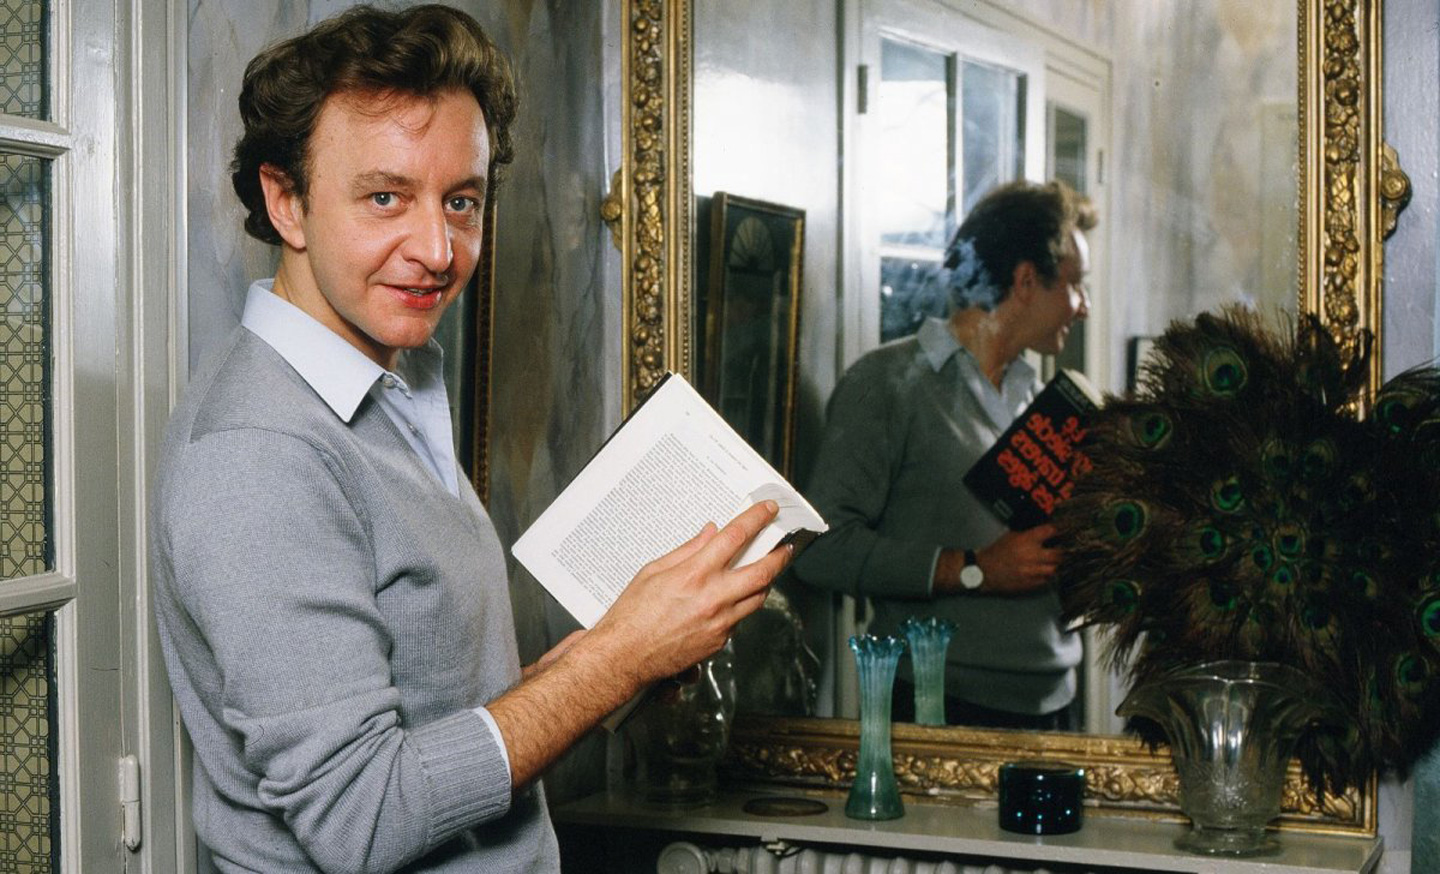
\includegraphics[width=14cm]{res/muray.jpg}
	}
\end{center}

Philippe Muray, born on June 10\textsuperscript{th} 1945 in Angers and deceased March 2\textsuperscript{nd} 2006 in Paris, was a French essayist and novelist known for his great talent as a polemist. He was married to Anne Muray.

\end{document}